%%%%%%%%%%%%%%%%%%%%%%% file template.tex %%%%%%%%%%%%%%%%%%%%%%%%%
%
% This is a general template file for the LaTeX package SVJour3
% for Springer journals.          Springer Heidelberg 2010/09/16
%
% Copy it to a new file with a new name and use it as the basis
% for your article. Delete % signs as needed.
%
% This template includes a few options for different layouts and
% content for various journals. Please consult a previous issue of
% your journal as needed.
%
%%%%%%%%%%%%%%%%%%%%%%%%%%%%%%%%%%%%%%%%%%%%%%%%%%%%%%%%%%%%%%%%%%%
%
% First comes an example EPS file -- just ignore it and
% proceed on the \documentclass line
% your LaTeX will extract the file if required
%
\RequirePackage{fix-cm}
%
%\documentclass{svjour3}                     % onecolumn (standard format)
%\documentclass[smallcondensed]{svjour3}     % onecolumn (ditto)
\documentclass[smallextended]{svjour3}       % onecolumn (second format)
%\documentclass[twocolumn]{svjour3}          % twocolumn
%
\smartqed  % flush right qed marks, e.g. at end of proof
%
\usepackage{amsmath}
\usepackage{booktabs}
\usepackage{subcaption}
\usepackage{tabularx}
\usepackage{nicefrac}
\usepackage[usenames]{xcolor}
\usepackage{lineno,hyperref}
\usepackage{graphicx}
%
% \usepackage{mathptmx}      % use Times fonts if available on your TeX system
%
% insert here the call for the packages your document requires
%\usepackage{latexsym}
% etc.
%
% please place your own definitions here and don't use \def but
% \newcommand{}{}
%
% Insert the name of "your journal" with
% \journalname{myjournal}
%
\begin{document}

\title{Formation of transverse cracks from the growth of multiple adjacent debonds on consecutive fibers in UD composites under transverse loading: Effect of the mutual position of debonds on Energy Release Rate
}
%\subtitle{}

%\titlerunning{Short form of title}        % if too long for running head

\author{Luca Di Stasio   \and
        Janis Varna \and
        Zoubir Ayadi
}

%\authorrunning{Short form of author list} % if too long for running head

\institute{Luca Di Stasio \at
              Lule\aa\ University of Technology, University Campus, SE-97187 Lule\aa, Sweden\\
              Universit\'e de Lorraine, EEIGM, IJL, 6 Rue Bastien Lepage, F-54010 Nancy, France\\
              \email{luca.di.stasio@ltu.se}           %  \\
%             \emph{Present address:} of F. Author  %  if needed
           \and
           Janis Varna \at
              Lule\aa\ University of Technology, University Campus, SE-97187 Lule\aa, Sweden\\
              \email{janis.varna@ltu.se}
		\and
           Zoubir Ayadi \at
              Universit\'e de Lorraine, EEIGM, IJL, 6 Rue Bastien Lepage, F-54010 Nancy, France\\
              \email{zoubir.ayadi@univ-lorraine.fr}
}

\date{Received: date / Accepted: date}
% The correct dates will be entered by the editor


\maketitle

\begin{abstract}
Models of Repeating Unit Cell (RUC) are developed to represent different Representative Volume Elements (RVEs) of UD composites of infinite size. Several damage states are studied in the form of different geometrical configurations of partially debonded and fully bonded fibers. It is found that the energetically most favorable cases for fiber/matrix interface crack (debond) growth are those where debonds grow on vertically (i.e. along thickness direction) aligned fibers. A maximum of Energy Release Rate (ERR) magnification is found when the vertically aligned partially debonded fibers are also contiguous. 
\keywords{Polymer-matrix Composites (PMCs) \and Transverse Failure \and Debonding \and Finite Element Analysis (FEA)}
% \PACS{PACS code1 \and PACS code2 \and more}
% \subclass{MSC code1 \and MSC code2 \and more}
\end{abstract}

%%%%%%%%%%%%%%%%%%%%%%%%%%%%%%%%%%%%%%%%%%%%%%%%%%%%%%%%%
%  INTRODUCTION
%%%%%%%%%%%%%%%%%%%%%%%%%%%%%%%%%%%%%%%%%%%%%%%%%%%%%%%%%

\section{Introduction}

The process of damage onset and development in multi-axial Fiber Reinforced Polymer Composite (FRPC) laminates involves several fracture mechanisms, which concur to the final failure of the composite part. Upon loading, one of the first macroscopic mode of damage is the occurrence in transverse cracks in plies where fibers are not aligned with the remote applied loading. A single transverse crack does not significantly compromise the load-carrying of the laminate, but in large numbers transverse cracks become detrimental to the elastic response of the part under loading. Furthermore, high concentrantions of transverse cracks lead to stress re-distribution and stress concentrations that can promote other more dangerous mode of fracture, quickly leading to the global failure of the laminate or part. Understanding the factors that influence transverse cracks onset and propagation is thus fundamental to improve current laminate design and to identify mechanisms of controlled propagation, delay and suppression of transverse cracks. This would provide toughness to FRPC laminates and help to avoid early part replacement, and thus waste, currently in use to prevent sudden catastrophic brittle failure.\\
Early microscopic observations in glass fiber-epoxy cross-ply laminates determined that onset of transverse cracking occurs at the microscopic level in the form of fiber-matrix interface cracks (or debonds)~\cite{Bailey1981}. Debonds grow along the arc direction of the fiber until reaching a critical size, then kink out of the interface and coalesce with other debonds across the ply thickness~\cite{Zhang1997}. Once a through-the-thickness crack tunnels through the width of the laminate, a transverse crack is formed. Formation and growth of debonds at the microscale thus play a key role in the overall process of initiation of transverse cracking. To improve our understanding of the latter, the former must be studied and modeled.\\
The first investigations on the mechanics of fiber/matrix debonding proposed analytical models of a single partially debonded fiber placed in an infinite matrix. These models focused on understanding the effect of the elastic properties mismatch between fiber and matrix. They were firstly solved by Perlman and Sih~\cite{Perlman1967}, who provided the solution in terms of stress and displacement fields, and Toya~\cite{Toya1974}, who evaluated the Energy Release Rate (ERR) at the debond tip. A closed-form analytical solution could only be found for the \textit{open crack} case, which assumes that no contact between debond faces occurs. This solution was shown to provide, for large debonds, a non-physical solution that implies inter-penetration of crack faces~\cite{Toya1974,Comninou1977}. Numerical treatment of the problem soon followed, in particular with the Boundary Element Method (BEM) solution by Paris et al.~\cite{Paris1996}. The numerical analysis of the single fiber model allowed first to understand the importance of crack face contact in the mechanics of fiber/matrix debonding~\cite{Varna1997a}, confirming earlier results regarding the straight bi-material interface crack~\cite{Comninou1977}. The process of fiber/matrix debonding was investigated in models of a single partially debonded fiber embedded in an effectively infinite matrix under remote tension~\cite{Paris1996} and remote compression~\cite{Correa2007}. Residual thermal stresses were also analyzed~\cite{Correa2011}. The effect of a second nearby fiber was studied, under different uniaxial and biaxial tensile and compressive applied loads~\cite{Correa2013,Correa2014,Sandino2016,Sandino2018}. Debond growth in a hexagonal cluster of fibers embedded in an effectively homogenized UD composite was investigated by Zhuang et al.~\cite{Zhuang2018}. The interaction of two debonds facing each other on two nearby fibers was addressed in~\cite{Varna2017} for a cluster of fibers immersed in a homogenized UD.\\
Models of kinking were developed for a single fiber in an infinite matrix~\cite{Paris2007} and a partially debonded fiber in a cluster of fibers inside a homogenized UD~\cite{Zhuang2018a}. A study on linking of debonds was proposed in~\cite{Varna2017}.\\
An analysis of the configuration preceding kinking and linking thus seems to lacking in the literature. We devote our attention in this paper to the analysis of Representative Volume Elements (RVEs) which model the presence of muliple debonds on fibers aligned across the thickness of UD composites. We focus on understanding the effect of the mutual interaction of consecutive debonds in the vertical direction and of their relative position, i.e. on the same or opposite sides of their respective fibers. We are interested in identifying which mechanisms might favor debond growth and which might, on the other hand, prevent it. For this reason, we select a regular arrangement of fibers and we adopt the approach of Linear Elastic Fracture Mechanics (LEFM) to characterize debond growth, by evaluating Mode I and Mode II Energy Release Rate (ERR). The Finite Element Method (FEM) is chosen to compute stress, strain and displacement fields, which are required to estimate ERR. The characteristics of the RVEs and the Finite Element (FE) solution are described in Sec.~\ref{sec:rveFem}; the main results are reported and discussed in Sec.~\ref{sec:results} and the main conclusions presented in Sec.~\ref{sec:conclusions}.

%%%%%%%%%%%%%%%%%%%%%%%%%%%%%%%%%%%%%%%%%%%%%%%%%%%%%%%%%
%  RVE MODELS AND FE DISCRETIZATION
%%%%%%%%%%%%%%%%%%%%%%%%%%%%%%%%%%%%%%%%%%%%%%%%%%%%%%%%%

\section{RVE models \& FE discretization}\label{sec:rveFem}

\subsection{Introduction \& Nomenclature}\label{subsec:names}

We focus in this article on debond growth in unidirectional (UD) composites subjected to in-plane transverse tensile loading. In particular, the interaction between debonds is studied through the development of models of Repeating Unit Cells (RUC) of laminates (see Fig.~\ref{fig:laminateModelsA} to Fig.~\ref{fig:laminateModelsC}). Only the central fiber in the RUC cell is in a damaged state in the form of a debond. The composite RUC is repeating both in the in-plane transverse direction and in the composite thickness direction; it thus corresponds to an infinite composite which models, in a limiting case, the behavior of a thick UD composite (free surfaces very far from the debonds). According to the proposed RUC design, the composite with debonds is considered as a sequence of stacked damaged and undamaged fiber rows, with each row having only one fiber in the thickness direction. Given that all the RUCs are characterized by a regular microstructure with fibers organized in a square-packing arrangement, they are as well Representative Volume Elements (RVE) of composites with a specific spatial distribution of debonds. In order to facilitate the treatment of models, let us introduce the in-plane coordinates $x$ and $y$, where $x$ is in the transverse direction of the UD composite ($z$ is consequently the through-the-thickness direction). Two considerations lie at the basis of the chosen RVE models. First, upon application of a load in the $x$-direction, the strain response in the $y$-direction is small due to the very small minor Poisson's ratio of the UD composite. Second, debonds are considered to be significantly longer in the fiber longitudinal direction than in the arc direction. We therefore use 2D models under the assumption of plane strain and defined in the $x-z$ section of the composite.  The analysis presented applies to long debonds and focuses on understanding the mechanisms of growth along the arc direction. Transverse tensile strain is applied to the composites in the form of a constant displacement in the $x$-direction along the vertical boundary of the RUC as shown in  Figures~\ref{fig:laminateModelsA} to~\ref{fig:modelschem}. As models are distinguished by the number of rows of fibers and by the spacing between debonds along the vertical and horizontal directions, the corresponding RUCs can be categorized based on the number $n$ of fibers in the horizontal direction and $k$ in the vertical direction. Vertical displacement coupling is always applied along the free surfaces. Thus. we introduce the common notation $n\times k-coupling$ to denote a RUC with $n\times k$ fibers and kinematic coupling applied to it. In Section~\ref{subsec:rve}, a detailed account of the selected combinations of $n$, $k$, and boundary conditions is provided as well as a description of the corresponding models of damaged composite.

\subsection{Models of Representative Volume Element (RVE) and equivalent boundary conditions}\label{subsec:rve}

The model shown in Fig.~\ref{fig:laminateModelsA} represents an infinite UD laminate in which debonds appear regularly every $n^{th}$ undamaged fiber in horizontal fiber rows and fiber rows containing damaged fibers appear every $k^{th}$ row of only undamaged fibers. The model is used to study the interaction between debonds appearing at regular but potentially different intervals along the horizontal and vertical direction, measured in terms of fully bonded (undamaged) fibers present between them. By changing the value of parameters $n$ and $k$ (number of fibers respectively in the horizontal and vertical direction) different distribution of debonds can be investigated: from isolated debonds far apart from each other (early stages of damage) to a UD with all the fibers partially debonded (an unphysical limit case). The model of Fig.~\ref{fig:laminateModelsA} is referred to as $n\times k-coupling$.

\begin{figure}[!h]
\centering
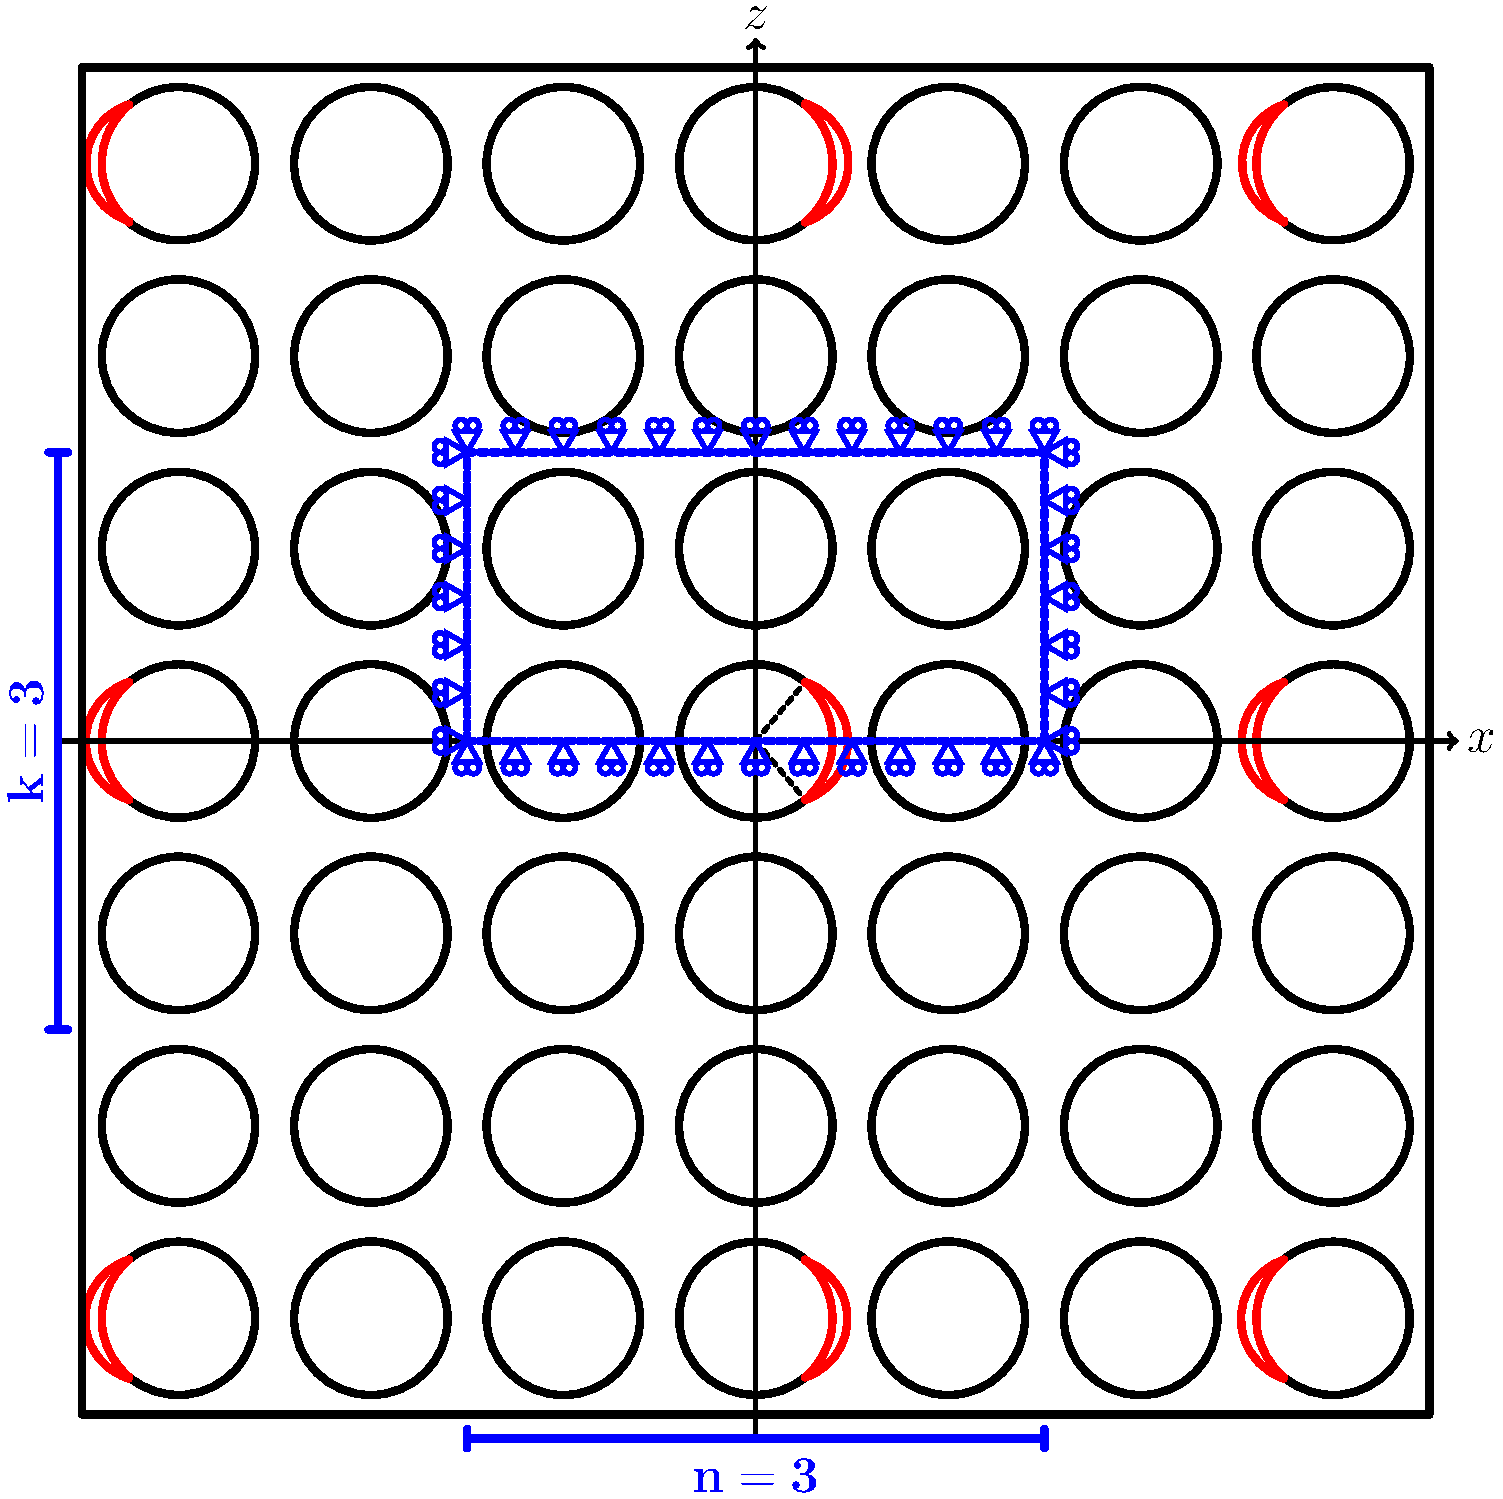
\includegraphics[width=\textwidth]{coupling.pdf}
\caption{Representative Volume Element $n\times k-symm$ of a UD composite with debonds appearing after $n-1$ and after $k-1$ undamaged fibers respectively in the horizontal and vertical direction. In the vertical direction, on fibers belonging to the same ``column'', debonds are located always on the same side.}\label{fig:laminateModelsA}
\end{figure}

Models in Figures~\ref{fig:laminateModelsB} and~\ref{fig:laminateModelsC} represent instead a UD composite with respectively vertical lines and horizontal rows of partially debonded fibers repeating at the regular intervals respectively in the horizontal and vertical direction, measured respectively in terms of vertical lines and horizontal rows of fully bonded (undamaged) fibers. According to the nomenclature introduced in Section~\ref{subsec:names}, these two models are identified respectively by $n\times 1-coupling$ and $1\times k-coupling$.

\begin{figure}[!h]
\centering
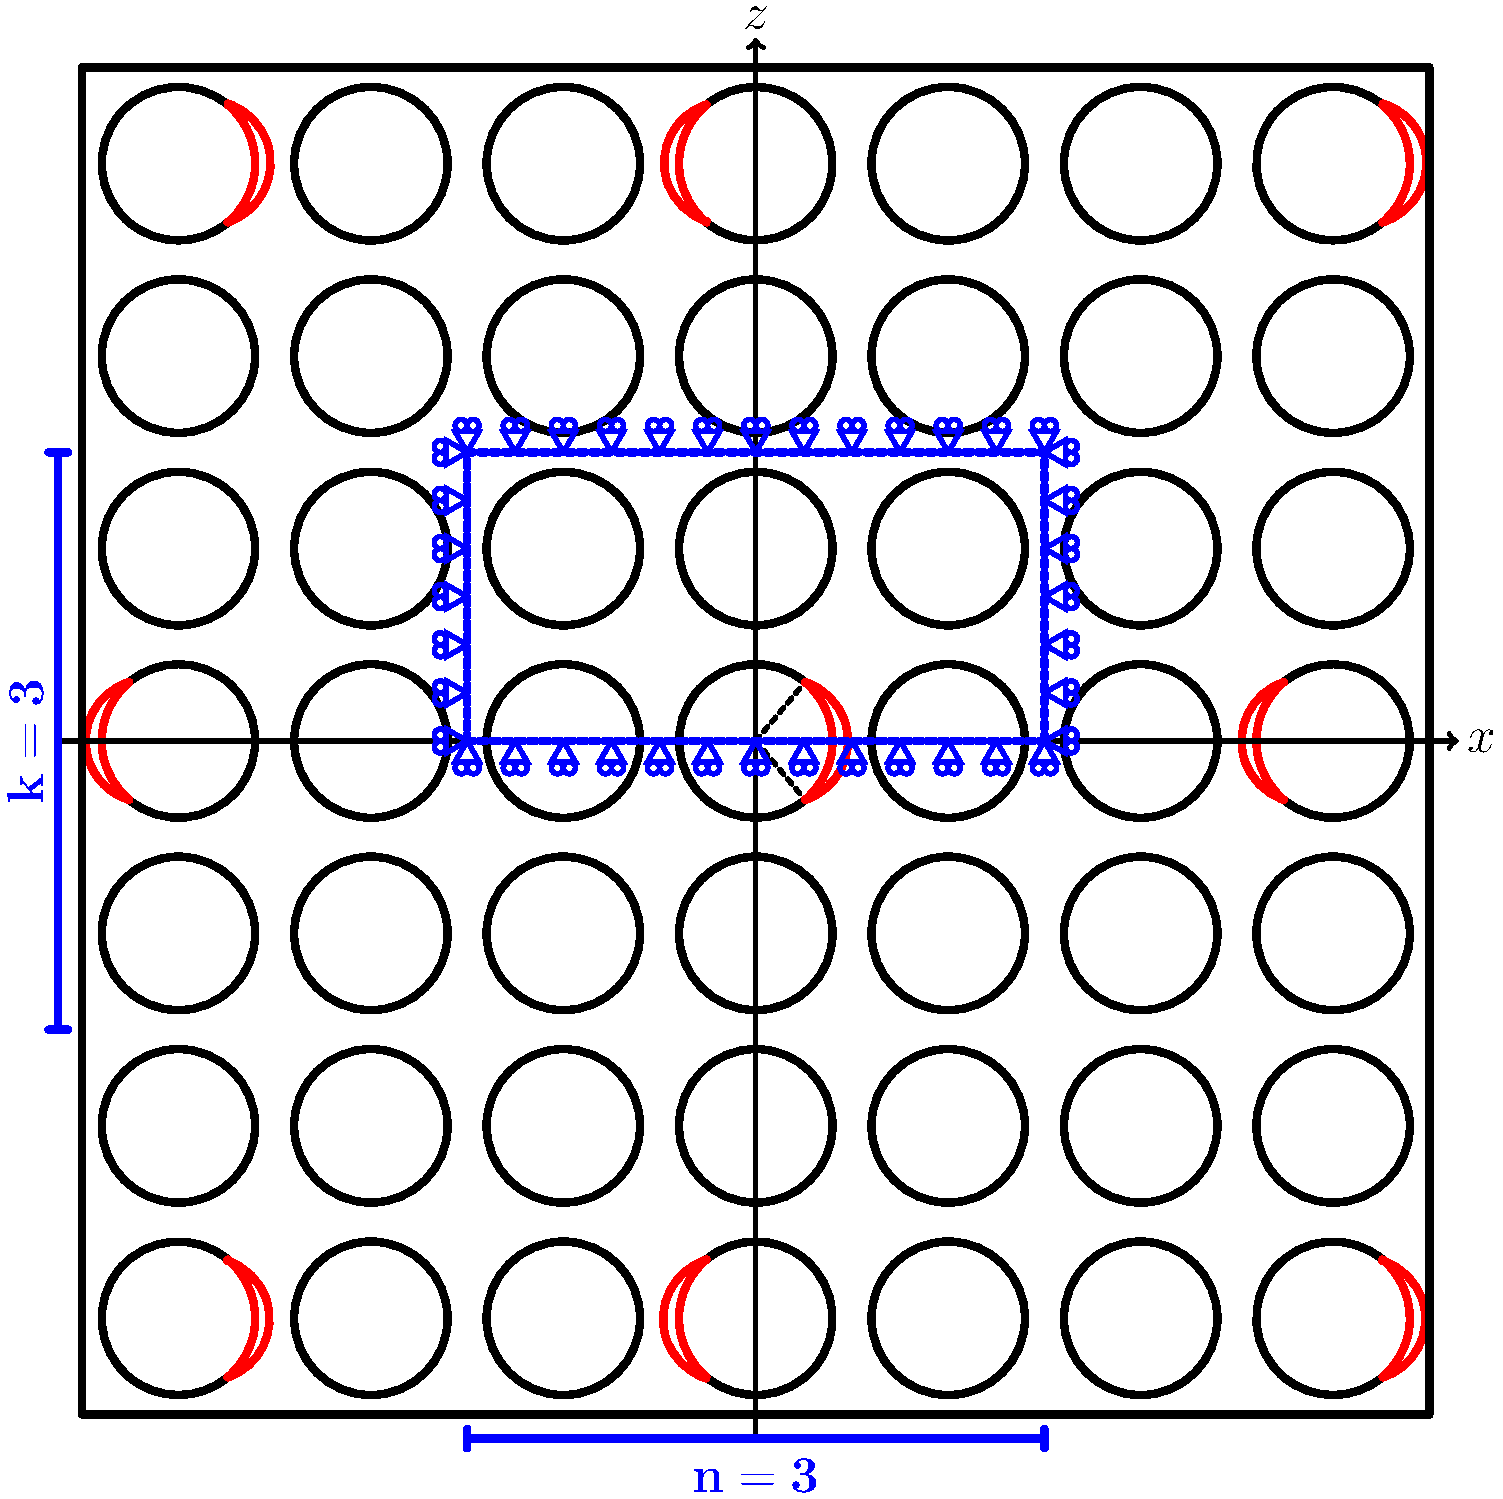
\includegraphics[width=\textwidth]{asymm.pdf}
\caption{Representative Volume Element $n\times k-asymm$  of a UD composite with debonds appearing after $n-1$ and after $k-1$ undamaged fibers respectively in the horizontal and vertical direction. In the vertical direction, on fibers belonging to the same ``column'', debonds are located on the opposite sides of consecutive fibers.}\label{fig:laminateModelsB}
\end{figure}

Model $n\times 1-coupling$ in Figure~\ref{fig:laminateModelsB} is studied to investigate the interaction of debonds in a configuration that represents, although in an idealized form, the stage preceding coalescence of debonds and formation of macroscopic transverse cracks. 
On the other hand, model $n\times 1-coupling$ in Figure~\ref{fig:laminateModelsC} addresses a configuration of debonds that has not been observed in in-situ analyses of UD composites in transverse tension and can thus be deemed unphysical, but has nonetheless the potential to shed light on debonds' interaction mechanisms that makes this configuration unobservable.

\subsection{Finite Element (FE) discretization}

Discretization and analysis of RUCs is performed with the Finite Element Method (FEM) within the Abaqus environment, a commercial FEM software~\cite{abq12}. Length $l$ and height $h$ of the model are respectively determined by the number of fibers $n$ in the horizontal direction and $k$ across the thickness (see Sec.~\ref{subsec:rve}) according to Eq.~\ref{eq:lengthheight}:

\begin{equation}\label{eq:lengthheight}
l=2nL\qquad h=kL;
\end{equation}

where $2L$ is the length of a one-fiber unit, see Fig.~\ref{fig:modelschem}, and $L$ is defined as a function of the fiber volume fraction $V_{f}$ and the fiber radius $R_{f}$ according to

\begin{equation}\label{eq:LVf}
L=\frac{R_{f}}{2}\sqrt{\frac{\pi}{V_{f}}}.
\end{equation}

$R_{f}$ is assumed to be the same for every fiber and equal to $1\ \mu m$. The choice of the previous value is not dictated by physical considerations but for simplicity. It is thus useful to remark here that, in a linear elastic solution as the one considered in the present work, the ERR is proportional to the geometrical dimensions of the model and, consequently, recalculation of the ERR for fibers of any size requires a simple multiplication. Notice also that relationships in Eqs.~\ref{eq:lengthheight} and~\ref{eq:LVf} imply that the local and global $V_{f}$ are everywhere equal.

\begin{figure}[!h]
\centering
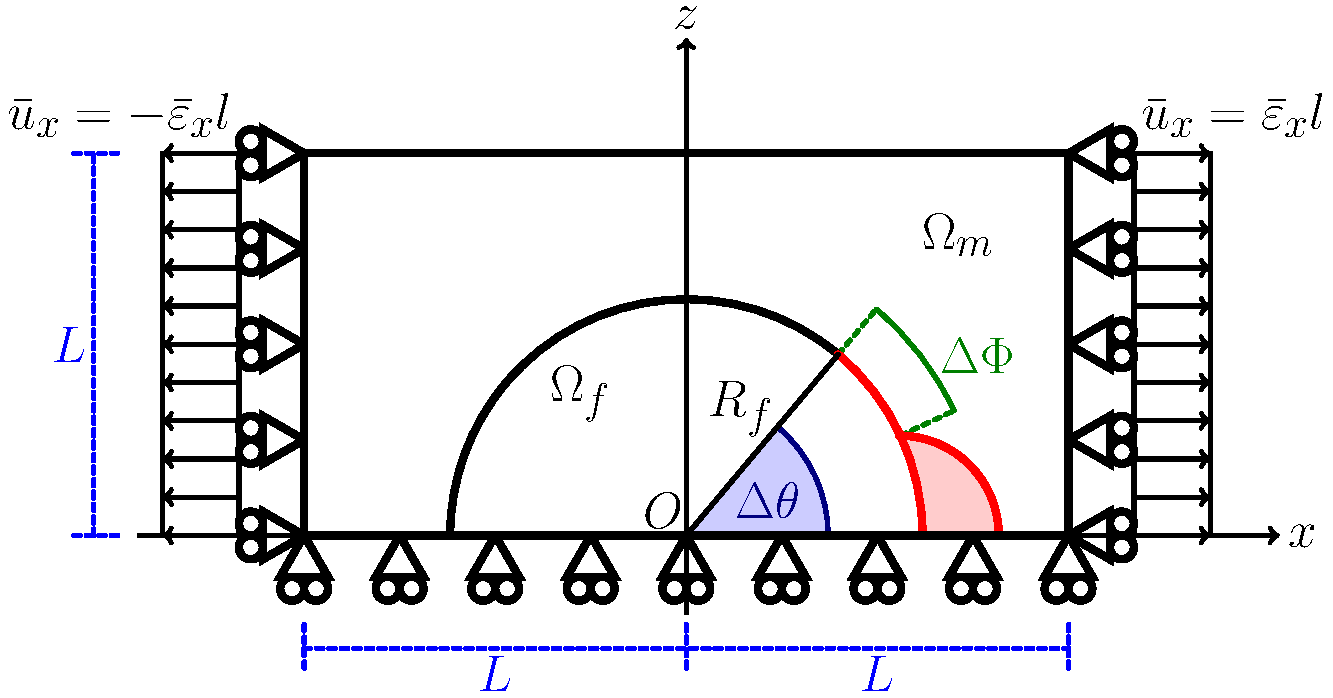
\includegraphics[width=\textwidth]{RUC.pdf}
\caption{Schematic of the model with its main parameters.}\label{fig:modelschem}
\end{figure}

The debond is placed symmetrically with respect to the $x$ axis (see Fig.~\ref{fig:modelschem}) and it is characterized by an angular size of $\Delta\theta$ (making the full debond size equal to $2\Delta\theta$). For large debond sizes (at least $\geq 60^{\circ}-80^{\circ}$), a region $\Delta\Phi$ of variable size appears at the crack tip where the crack faces are in contact with each other but free to slide relatively to each other. In order to model crack faces motion in the contact zone, frictionless contact is considered between the two crack faces to allow free sliding and avoid interpenetration. Symmetry with respect to the $x$ axis is applied on the lower boundary and coupling of vertical displacement on the upper boundary. Kinematic coupling on the $x$-displacement is applied along the left and right sides of the RUC in the form of a constant $x$-displacement $\pm\bar{\varepsilon}_{x} l$, corresponding to transverse strain $\bar{\varepsilon}_{x}$ equal to $1\%$.

\begin{table}[!htbp]
 \centering
 \caption{Summary of the mechanical properties of fiber and matrix. $E$ stands for Young's modulus, $\mu$ for shear modulus and $\nu$ for Poisson's ratio.}
 \begin{tabular}{cccc}
\textbf{Material} & \textbf{$E\left[GPa\right]$}\ & \textbf{$\mu\left[GPa\right]$} & \textbf{$\nu\left[-\right]$} \\
\midrule
Glass fiber    & 70.0  & 29.2   & 0.2  \\
Epoxy    & 3.5    & 1.25   & 0.4
\end{tabular}
\label{tab:phaseprop}
\end{table}

Meshing of the model is accomplished with second order, 2D, plane strain triangular (CPE6) and quadrilateral (CPE8) elements. A regular mesh of 8-node ($2^{nd}$ order rectangular) elements with almost unitary aspect ratio is enforced at the crack tip in order to ensure the convergence of the ERR. The angular size $\delta$ of an element in the crack tip neighborhood is always equal to $0.05^{\circ}$. The crack faces are modeled as element-based surfaces and a small-sliding contact pair interaction with no friction is imposed between them. The Mode I, Mode II and total Energy Release Rates (ERRs) (respectively referred to as $G_{I}$, $G_{II}$ and $G_{TOT}$) are the main result of FEM simulations; they are evaluated using the VCCT~\cite{Krueger2004} implemented in a in-house Python routine and, for $G_{TOT}$ only, the J-integral~\cite{Rice1968} is calculated by use of the Abaqus built-in command. A glass fiber-epoxy UD composite is treated in the present work, and it is assumed that their response lies always in the linear elastic domain. The material properties of glass fiber and epoxy are reported in Table~\ref{tab:phaseprop}. Validation is performed with respect to the results reported in~\cite{Paris2007,Sandino2016}, which were obtained with the Boundary Element Method (BEM) for a model of a single fiber with a symmetric debond placed in an infinite matrix. As discussed in more detail in~\cite{DiStasio2019}, the agreement between FEM (present work) and BEM~\cite{Paris2007,Sandino2016} solutions is good and the difference between the two does not exceed $5\%$. This provides us with a level of uncertainty with which we can analyze the significance of observed trends: any relative difference in ERR between different RUCs smaller than $5\%$ cannot be reliably distinguished from numerical uncertainty and its discussion should thus be avoided.

\section{Results \& Discussion}\label{sec:results}

\subsection{Interaction between isolated debonds in infinite UD composites}\label{subsec:chesstable}

The effect on Mode I and Mode II ERR of the interaction between debonds appearing at regular distances (in terms of fully bonded fibers) in the horizontal and vertical directions (models $n\times k-coupling$) is shown respectively in Figure~\ref{fig:debonddebondGI} and Figure~\ref{fig:debonddebondGII}. It can be observed that it is the distance between debonds in the horizontal direction that presents a relevant effect on ERR: the number of fully bonded fibers between consecutive debonds in the vertical direction has a negligible influence on Mode I and a very modest effect, below or at the limit of the $5\%$ accuracy of the model, on Mode II.

\begin{figure}[!h]
\centering
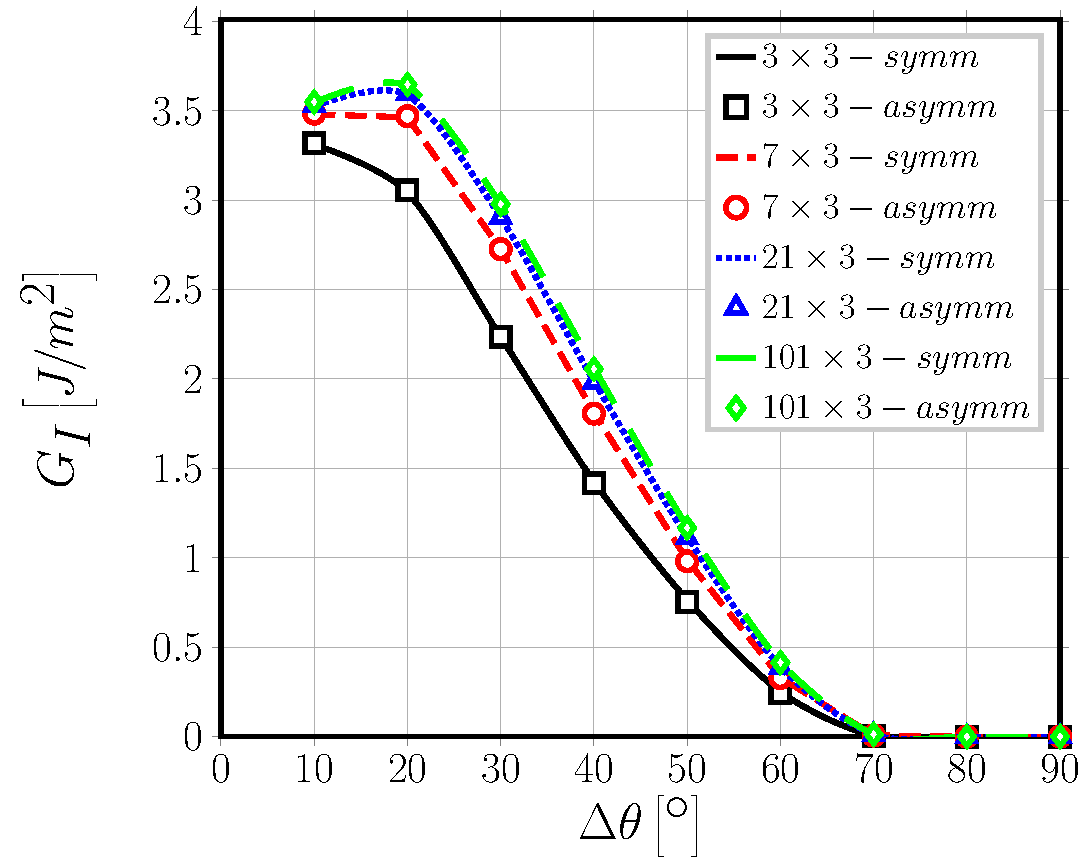
\includegraphics[width=\textwidth]{nxk-coupling-vf60-GI.pdf}
\caption{Effect of debond-debond interaction in infinite UD composites on Mode I ERR: models $n\times k-coupling$. $V_{f}=60\%$, $\varepsilon_{x}=1\%$.}\label{fig:debonddebondGI}
\end{figure}

On the other hand, increasing the number of fully bonded fibers between debonds in the horizontal direction leads to a significant increase in both Mode I and Mode II ERR, due to the magnification of the $x$-strain in the crack tip neighborhood~\cite{DiStasio2019}. A critical distance (in terms of undamaged fibers) at which a non-interacting solution can be observed is apparent for Mode I (Figure~\ref{fig:debonddebondGI}). Given that Mode II ERR for models $21\times 3-coupling$, $21\times 21-coupling$, $101\times 3-coupling$ and $101\times 101-coupling$ is in a $\leq5\%$ range with respect to each other and thus their difference is not significant taking into account model accuracy, it can be argued that also in Mode II a critical distance exists at which a non-interacting solution appears.

\begin{figure}[!h]
\centering
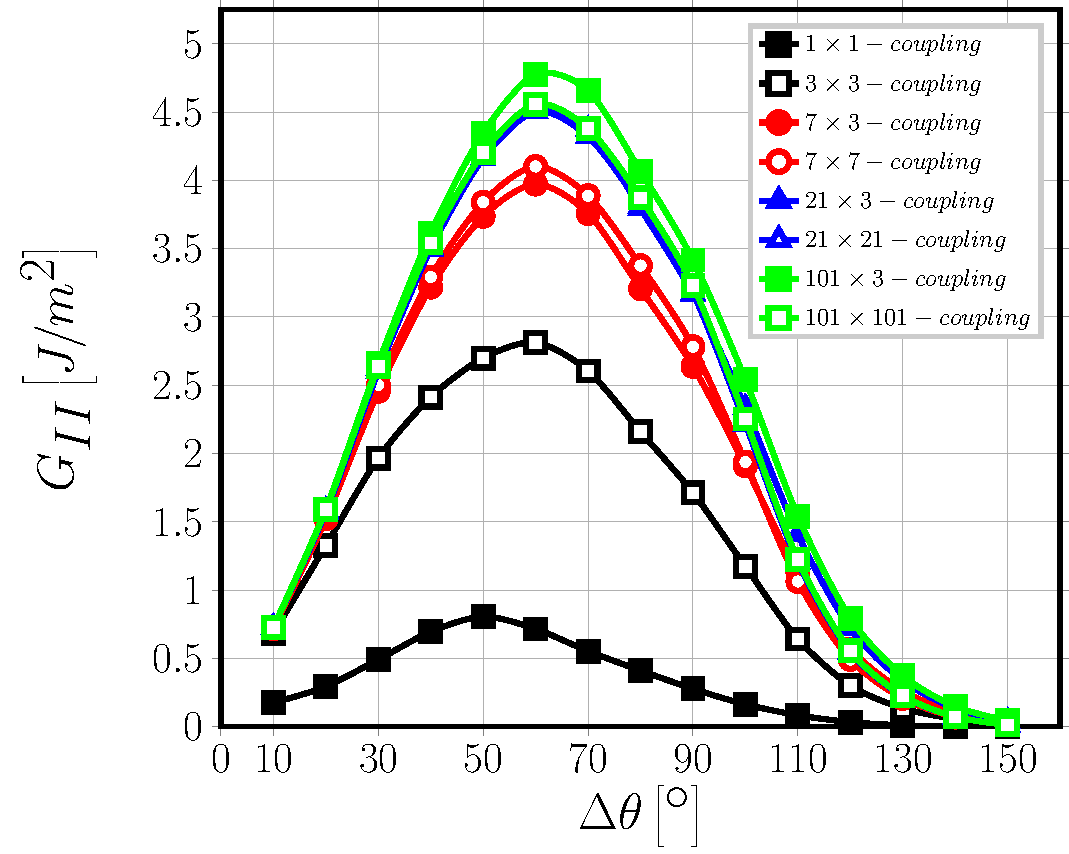
\includegraphics[width=\textwidth]{nxk-coupling-vf60-GII.pdf}
\caption{Effect of debond-debond interaction in infinite UD composites on Mode II ERR: models $n\times k-coupling$. $V_{f}=60\%$, $\varepsilon_{x}=1\%$.}\label{fig:debonddebondGII}
\end{figure}

\subsection{Debond-debond interaction between horizontal rows of partially debonded fibers in infinite UD composites}\label{subsec:horizontal}

The results presented in Figures~\ref{fig:horizontalGI} and~\ref{fig:horizontalGII} for respectively Mode I and Mode II ERR of models $1\times k-coupling$ confirm the observations presented in Section~\ref{subsec:chesstable}. Models $1\times k-coupling$ represents the RVE of an infinite UD composite with horizontal fiber rows that appear at regular intervals (measured in terms of fully bonded fibers) and in which fibers are all partially debonded (see Fig.~\ref{fig:laminateModelsC} for reference).

\begin{figure}[!h]
\centering
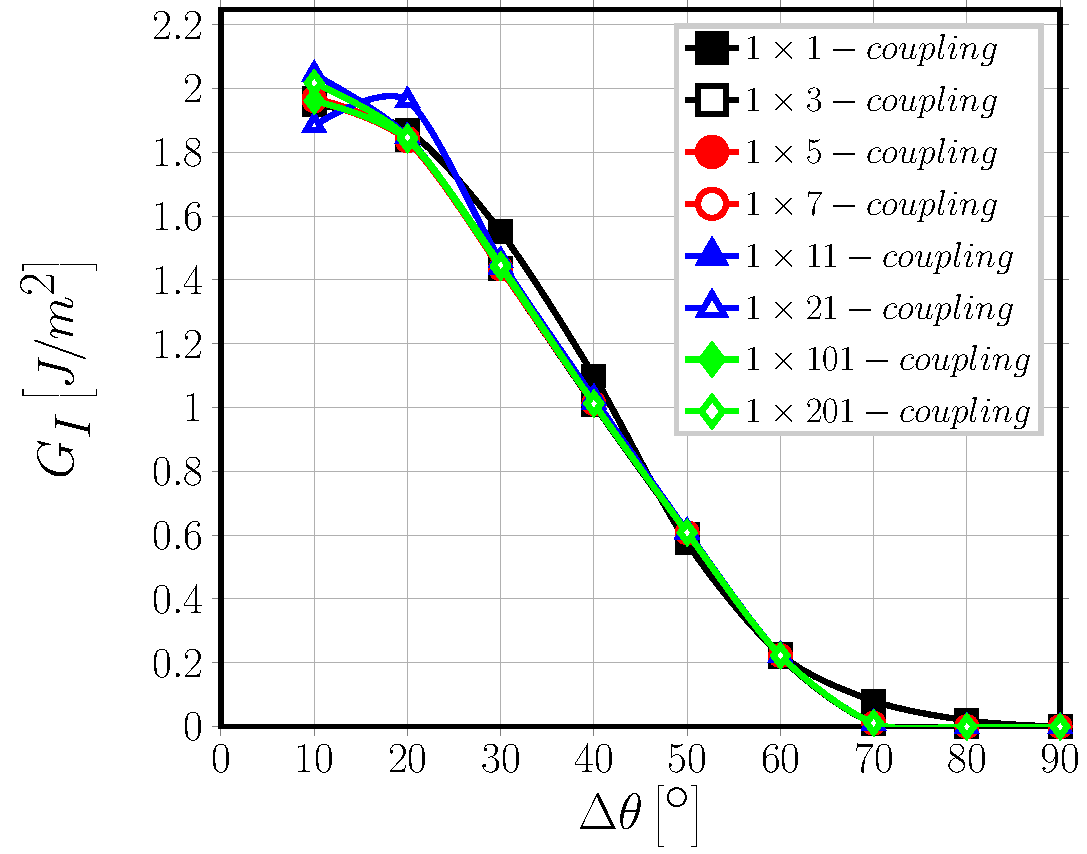
\includegraphics[width=\textwidth]{1xk-coupling-vf60-GI.pdf}
\caption{Effect of debond-debond interaction in infinite UD composites on Mode I ERR: models $1\times k-coupling$. $V_{f}=60\%$, $\varepsilon_{x}=1\%$.}\label{fig:horizontalGI}
\end{figure}

Varying the number $k$ of undamaged fibers between fiber rows of only partially debonded fibers does not have any effect on ERR, neither in Mode I (Figure~\ref{fig:horizontalGI}) nor in Mode II (Figure~\ref{fig:horizontalGII}). The observations of Sec.~\ref{subsec:chesstable} are thus confirmed: it is the presence of fully bonded fibers only in the horizontal direction, i.e. the loading direction, that affects the debond ERR through $x$-strain magnification.

\begin{figure}[!h]
\centering
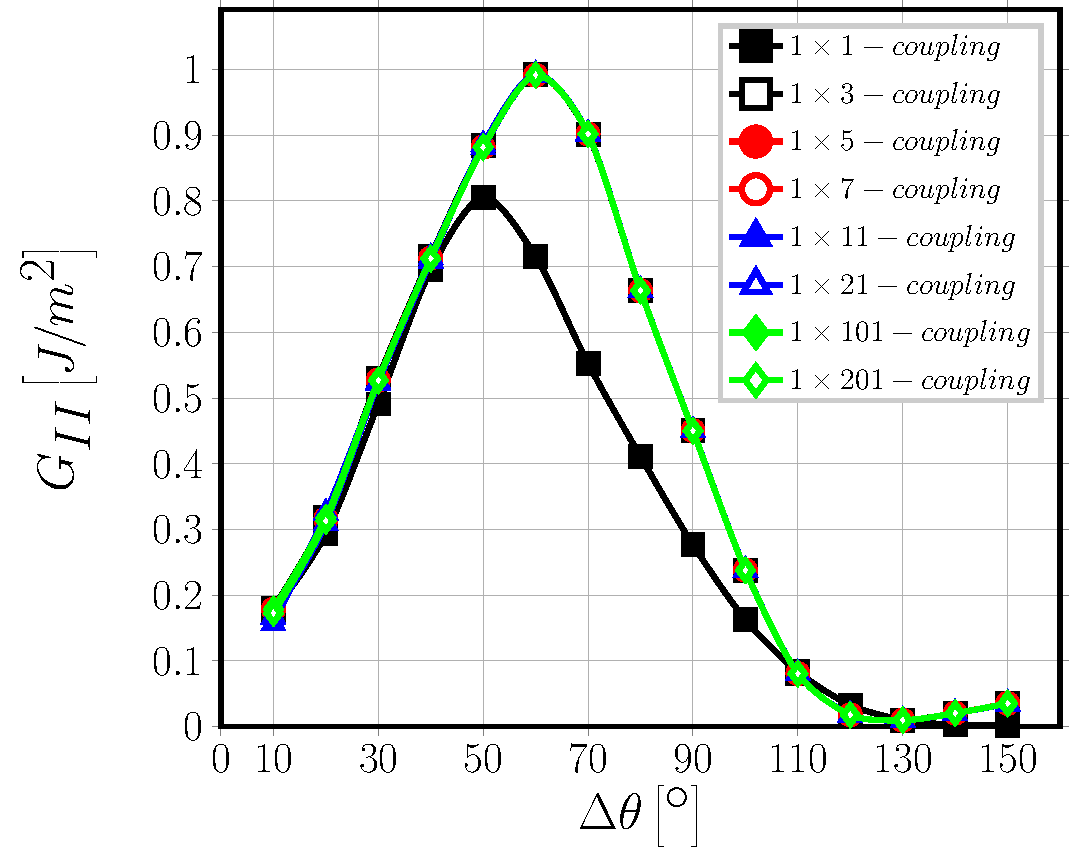
\includegraphics[width=\textwidth]{1xk-coupling-vf60-GII.pdf}
\caption{Effect of debond-debond interaction in infinite UD composites on Mode II ERR: models $1\times k-coupling$. $V_{f}=60\%$, $\varepsilon_{x}=1\%$.}\label{fig:horizontalGII}
\end{figure}

\subsection{Debond-debond interaction between vertical lines of partially debonded fibers in infinite UD composites}

Figures~\ref{fig:verticalGI} and~\ref{fig:verticalGII} report respectively Mode I and Mode II ERR for models $1\times k-coupling$, which correspond to the RVEs of UD composites with vertical lines of partially debonded fibers appearing at regular intervals (in terms of undamaged fibers) in the horizontal direction (see Fig.~\ref{fig:laminateModelsB} for reference). 

\begin{figure}[!h]
\centering
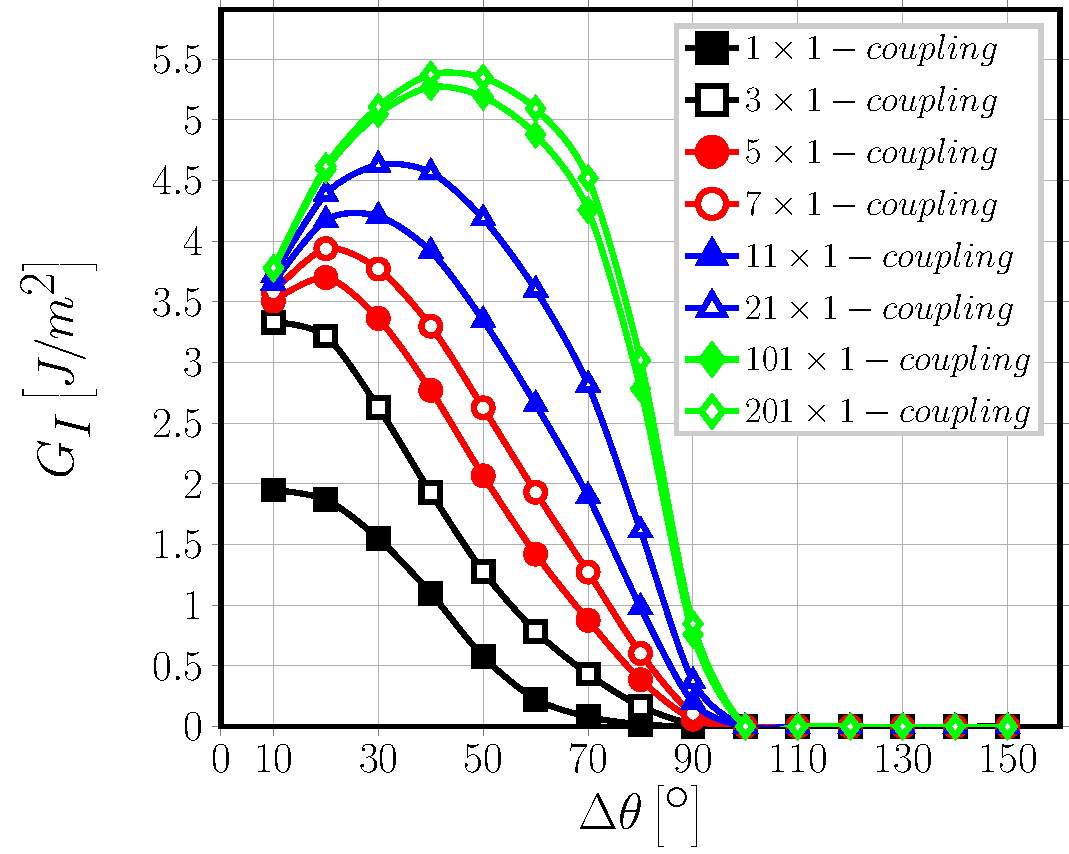
\includegraphics[width=\textwidth]{nx1-coupling-vf60-GI.pdf}
\caption{Effect of debond-debond interaction in infinite UD composites on Mode I ERR: models $n\times 1-coupling$. $V_{f}=60\%$, $\varepsilon_{x}=1\%$.}\label{fig:verticalGI}
\end{figure}

As it can be expected from the discussion of Sec.~\ref{subsec:chesstable} and Sec.~\ref{subsec:horizontal}, increasing the number of fully bonded fibers between two consecutive lines of partially debonded fibers is responsible for significant increases in both Mode I and Mode II ERR.

\begin{figure}[!h]
\centering
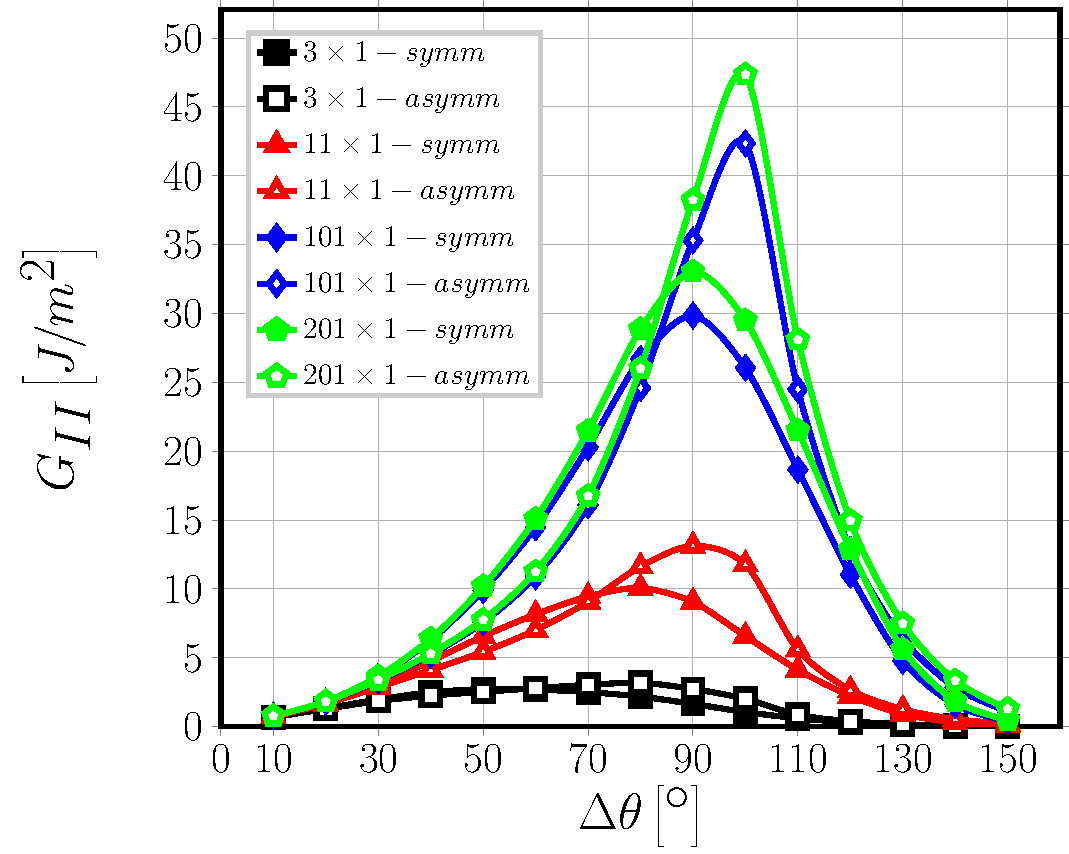
\includegraphics[width=\textwidth]{nx1-coupling-vf60-GII.pdf}
\caption{Effect of debond-debond interaction in infinite UD composites on Mode II ERR: models $n\times 1-coupling$. $V_{f}=60\%$, $\varepsilon_{x}=1\%$.}\label{fig:verticalGII}
\end{figure}

However, comparison of Fig.~\ref{fig:verticalGI} with Fig.~\ref{fig:horizontalGI} and of Fig.~\ref{fig:verticalGII} with Fig.~\ref{fig:horizontalGII} provides an additional interesting result: the presence of fully bonded fibers between debonds appearing on vertically aligned fibers reduces both $G_{I}$ and $G_{II}$. On the other hand, for the same horizontal distance between debonded fibers, the energetically most favorable configuration is achieved when debonds are contiguous along the vertical direction. Two further effects can be observed: the onset of the contact zone is delayed up to a debond size of $\sim100^{\circ}$ (Fig.~\ref{fig:verticalGI}); the peak value of $G_{II}$ is shifted to a debond size of up to $90^{\circ}$ (Fig.~\ref{fig:verticalGII}). Thus, larger debonds are in general favored. This behavior can be related to the local deformation of the matrix. Between two vertically aligned debonds, the matrix strip between the two partially debonded fibers has, locally, both the lower and the upper surface free to deform. Due to Poisson's effect, the two surfaces move towards each other, imposing an opening displacement on the crack tip. This in turn favors Mode I and delays the onset of the contact zone. Furthermore, taking into account that fibers are more rigid than the sorrounding matrix, when the fiber on top of the debonded one is undamaged (fully bonded), the $x$-displacement field in the matrix is restrained by the requirement of continuity at the interface. When instead another partially debonded fiber is present, a matrix strip is created with an upper and lower free surfaces, i.e. detached from the upper and lower fibers. The displacement field in this matrix strip is thus not restrained by the more rigid fibers and a magnification effect of the $x-strain$ takes place. This in turn causes an increase in $G_{I}$ for smaller debonds (the $x$-displacement is the major component of the crack opening displacement at the crack tip) and  in $G_{II}$ for larger ones (the $x$-displacement is the major component of the crack shear displacement at the crack tip).

\section{Conclusions}\label{sec:conclusions}

Different models of infinite UD composites have been studied with different configurations of multiple interacting debonds in order to investigate their effect of Mode I and Mode II Energy Release Rate.\\
Building upon the observations made in the previous section, several conclusions can be drawn about the growth of debonds in UD composites:

\begin{itemize}
\item at given strain level, multiple debonds can appear on not consecutive vertically-aligned fibers;
\item at a given strain level, the vertical lines of fibers on which debonds grow are determined by the horizontal distance from pre-existing debonds;
\item a minimum non-interactive distance exists for the Energy Release Rate;
\item when spacing between vertical lines of debonds is lower than the minimum non-interactive distance, the ERR decreases;
\item thus, conversely, when spacing between vertical lines of debonds is lower than the minimum non-interactive distance, higher levels of strain are needed to grow debonds;
\item growth of debonds appearing on contiguous vertically-aligned fibers is energetically the most favorable;
\item larger debonds are favored on contiguous vertically aligned partially debonded fibers.
\end{itemize}



\begin{acknowledgements}
Luca Di Stasio gratefully acknowledges the support of the European School of Materials (EUSMAT) through the DocMASE Doctoral Programme and the European Commission through the Erasmus Mundus Programme.
\end{acknowledgements}


% Authors must disclose all relationships or interests that 
% could have direct or potential influence or impart bias on 
% the work: 
%
% \section*{Conflict of interest}
%
% The authors declare that they have no conflict of interest.


% BibTeX users please use one of
%\bibliographystyle{spbasic}      % basic style, author-year citations
\bibliographystyle{spmpsci}      % mathematics and physical sciences
%\bibliographystyle{spphys}       % APS-like style for physics
\bibliography{refs}   % name your BibTeX data base

%% Non-BibTeX users please use
%\begin{thebibliography}{}
%%
%% and use \bibitem to create references. Consult the Instructions
%% for authors for reference list style.
%%
%\bibitem{RefJ}
%% Format for Journal Reference
%Author, Article title, Journal, Volume, page numbers (year)
%% Format for books
%\bibitem{RefB}
%Author, Book title, page numbers. Publisher, place (year)
%% etc
%\end{thebibliography}

\end{document}
% end of file template.tex

